\documentclass[letterpaper, paper,11pt]{AAS}	% for preprint proceedings
\usepackage{bm}
\usepackage{amsmath}
\usepackage{subfigure}
%\usepackage[notref,notcite]{showkeys}  % use this to temporarily show labels
\usepackage[colorlinks=true, pdfstartview=FitV, linkcolor=black, citecolor= black, urlcolor= black]{hyperref}
\usepackage{overcite}
\usepackage{footnpag}			      	% make footnote symbols restart on each page
% \usepackage{listings}                   % Code Listings
\usepackage[table, x11names]{xcolor}                     % Code Coloring
\usepackage{xfrac}                      % Slanted Fractions
\usepackage{booktabs}                   % Table Styling
\usepackage{multirow}                   % Table Styling
\usepackage{tikz}

% DEFINING CODE COLORS
% \definecolor{comments}{rgb}{0.0, 0.5, 0.0}
% \definecolor{keywords}{rgb}{0.01, 0.28, 1}

% ADDITIONAL COMMANDS
\newcommand*\circled[1]{\tikz[baseline=(char.base)]{
            \node[shape=circle,draw,inner sep=0.8pt] (char) {#1};}}

% \lstset{
%     basicstyle = \small\ttfamily,
%     language = Python,
%     frame = lines,
%     backgroundcolor = \color{lightgray!10},
%     commentstyle = \color{comments}\ttfamily\small,
%     keywordstyle = \color{keywords}\bf\ttfamily\small,
%     framesep=\fboxsep,
% }

\PaperNumber{20-686}

\begin{document}
\setcounter{page}{5199}

\title{Broad Trajectory Searches Using Monte Carlo Tree Search with the Inclusion of $\Delta$VEGA Trajectories}

\author{
    Burton A. Yale\thanks{Aerospace Engineering, Cal Poly Pomona, 3801 W Temple Ave., Pomona, California, 91786, USA}
        \thanks{Undergraduate Student, E-mail: bayale@cpp.edu},
    Rohan D. Patel\footnotemark[1]
        \thanks{Undergraduate Student, E-mail: rohanpatel@cpp.edu},
    Jehosafat J. Cabrera\footnotemark[1]
        \thanks{Undergraduate Student, E-mail: jehosafatc@cpp.edu},
    and Navid Nakhjiri\footnotemark[1]
        \thanks{Associate Professor, E-mail: nnakhjiri@cpp.edu}
}

\maketitle{}

\begin{abstract}
Multiple flybys of the inner planets and the application of $V_{\infty}$ leveraging are essential trajectory design techniques to reduce the required launch energy for interplanetary missions. These trajectories are often difficult to formulate and require extensive computational resources. However, this problem can be classified as a combinatorial task and can be solved by the Monte Carlo Tree Search (MCTS) method. In this paper, an MCTS algorithm is developed and tested. The tree search is able to incorporate $V_\infty$ leveraging of Earth ($\Delta V$EGA), which will allow the algorithm to find an additional set of feasible sequences. Several cases are optimized and the tree search's performance and accuracy is discussed. This algorithm will allow for the inner-planetary flyby search planning for outer planet missions.
\end{abstract}

\section*{Introduction}
\pdfbookmark[1]{Introduction}{intro}

Broad trajectory searches are one of the first steps in mission planning, allowing for the selection of candidate sequences given a list of constraints. As is the nature with combinatorial problems, every additional flyby adds another dimension to the search space. Brute force methods lead to expensive but thorough results. Also, by pruning possible choices before each selection, the overall computation time can be significantly decreased, at the expense of not finding all possible results. The method of interest for this paper is enumerated searches, a subset of grid searches, as recent work has proven their ability to quickly and accurately locate multi-leg interplanetary trajectories~\cite{Hennes2015}. \textbf{M}onte \textbf{C}arlo \textbf{T}ree \textbf{S}earch (MCTS) is a heuristics-based adaptation of the enumerated search and has the ability to both explore and exploit its environment. With this, it is possible for the algorithm to efficiently narrow down possible search paths for future iterations to explore. As such, larger search spaces can be employed without exponential growth in computation time. This algorithm will deliver a set of planetary sequences and the dates associated that meet mission criteria, such as destination planet, launch windows, total $\Delta V$ budgets, etc. The results from the tree search can then be passed to an optimizer for additional detail.

In this paper, we discuss and implement the MCTS method to the multi-flyby sequence problem. We consider Earth $V_\infty$ leveraging in the search space by approximating the required $\Delta V$ and flyby conditions of $\Delta V$EGA trajectories. We also demonstrate the capability of the algorithm to find ballistic or $\Delta V$EGA multi-flyby sequences to the outer planets.

\section*{Background}
\pdfbookmark[1]{Background}{bg}

Multi-flyby sequence generation begins with a set of target encounter bodies to visit and the evaluation of the feasibility of transfers between them. First, a sequence of encounter bodies is selected and is followed by evaluating all possible trajectories for that specified sequence. Due to the increasing complexity of gravity assists and combinatorial solutions, a low-fidelity tool is generally utilized first to map out the search space. Once a set of possible sequences and their respective encounter epochs are known, solutions of interest can be optimized in further detail. This is often referred to as pathfinding and path-solving, respectively~\cite{Hughes2016}. Pathfinding is a sequence optimization problem that provides a diverse set of mission options. Path-solving, on the other hand, embodies a trajectory optimization problem where two types of transfer models, low-thrust or multi-impulse, are mainly considered~\cite{Li2019}. Some common techniques for pathfinding and generating search spaces include evolutionary algorithms, machine learning, evolutionary neuro-controllers, and tree search methods~\cite{Izzo2019}.

Evolutionary algorithms are optimization routines that make use of heuristics and Darwinian evolution to solve complex optimization problems. Three popular types are genetic algorithms, Differential Evolution (DE), and Particle Swarm Optimization (PSO). DE has been successfully used as an optimization routine to design Halo Orbits, transfers to Halo Orbits, and as an interplanetary mission design algorithm~\cite{Nath2016, Olds2007}.  The Cassini and Galileo missions were considered as case studies to analyze the performance of these algorithms. The DE routine was able to come within appropriate bounds of both trajectories and found optimal sequences with the given flight constraints. PSO was used by Zhuang et al.~\cite{Zhuang2014} in combination with Legendre pseudo-spectral method for solving time-optimal trajectory planning problems. When considering non-evolutionary algorithms for pathfinding, a common method is the use of the grid-search technique. This has been previously used as a search method to find possible trajectories to Kuiper belt objects (KBOs)~\cite{Penas2019}. Grid search is a type of search algorithm with the ability to map the entire search space so that no regions of interest are missed. This method has been used to properly parameterize the time-of-flight between encounter bodies. It, however, can be expensive in terms of computing power and time. To alleviate both of these constraints, heuristics can be implemented. Beam Search (BS), a heuristic tree search algorithm, can be used as a method to find a sequence of planets for gravitational assists \cite{Penas2019}. BS uses the method of Breadth-First Search (BFS) to find the tree of possibilities. With each layer of the tree and orders the nodes in accordance with their heuristic cost. It only chooses the nodes with a maximum value to build from. Depth-First Search (DPS), alternatively, is used as a searching criterion to traverse down the tree~\cite{Izzo2013}. Contrary to BFS, DPS does not search the tree at every level but rather explores a branch until the termination criteria are met. After, it propagates up each parent node updating branches to start the process again. Both the BFS and DPS, search and prune the environmental choices consecutively. Using the Lazy Race Tree Search, the search space is pruned, and nodes ranked through the time of flight~\cite{Izzo2013}. The use of heuristics avoids finding redundant solutions and increases the efficiency of the method used. Izzo et al.~\cite{Hennes2015} proposed the use of the Monte Carlo Tree Search to find fast solutions to interplanetary trajectories.

Monte Carlo methods have been suggested extensively for games with random behavior and minimal observability. The nature of the Monte Carlo methods, however, allow them to be applied to deterministic games with faultless information~\cite{Browne2012}. Starting from the initial state, a large number of games and actions are simulated until the end of the game. In the majority of cases, actions are chosen at random with no link to the game theory. This fact implies that even if the iterative process is executed for an extended period of time, the move selected and path selected is not optimal. The search sensitivity criteria of DPS, BS, and BFS are explored in conjunction with that of the MCTS and compared. Currently, ballistic sequence finding search algorithms either cannot accommodate for large trajectory maneuvers, or would need to account for them with large discontinuous velocities between flyby sequences. This paper aims at incorporating a specific type of deep space maneuver, DVEGA, to return a more comprehensive search space.

\section*{Monte Carlo Tree Search Implementation}
\pdfbookmark[1]{Monte Carlo Tree Search Implementation}{mcts}

The tree is built upon a set of individual nodes, connected to each other through their parent and children, much like a family tree. Each node has a corresponding state to represent a leg in the trajectory of the spacecraft, with a planetary body, and the time at which it is encountered. As the algorithm builds the tree, the process can be characterized by four essential steps: \circled{1} selection,\hspace{1em} \circled{2} expansion, \circled{3} simulation, and \circled{4} backpropagation, as depicted in Figure~\ref*{fig:mctsFunc}.

At the initialization of the tree, an array of launch nodes is specified based upon user input. If the sample time span is larger than a year, the number of corresponding nodes will be modified in order to evenly sample the launch window. From this point, the algorithm will begin its core loop to search out possible trajectory sequences, until the user-defined iteration budget is depleted.

\begin{figure}[htb]
    \centering
    \begin{tikzpicture}
        \node[anchor=south west,inner sep=0] (image) at (0,0) {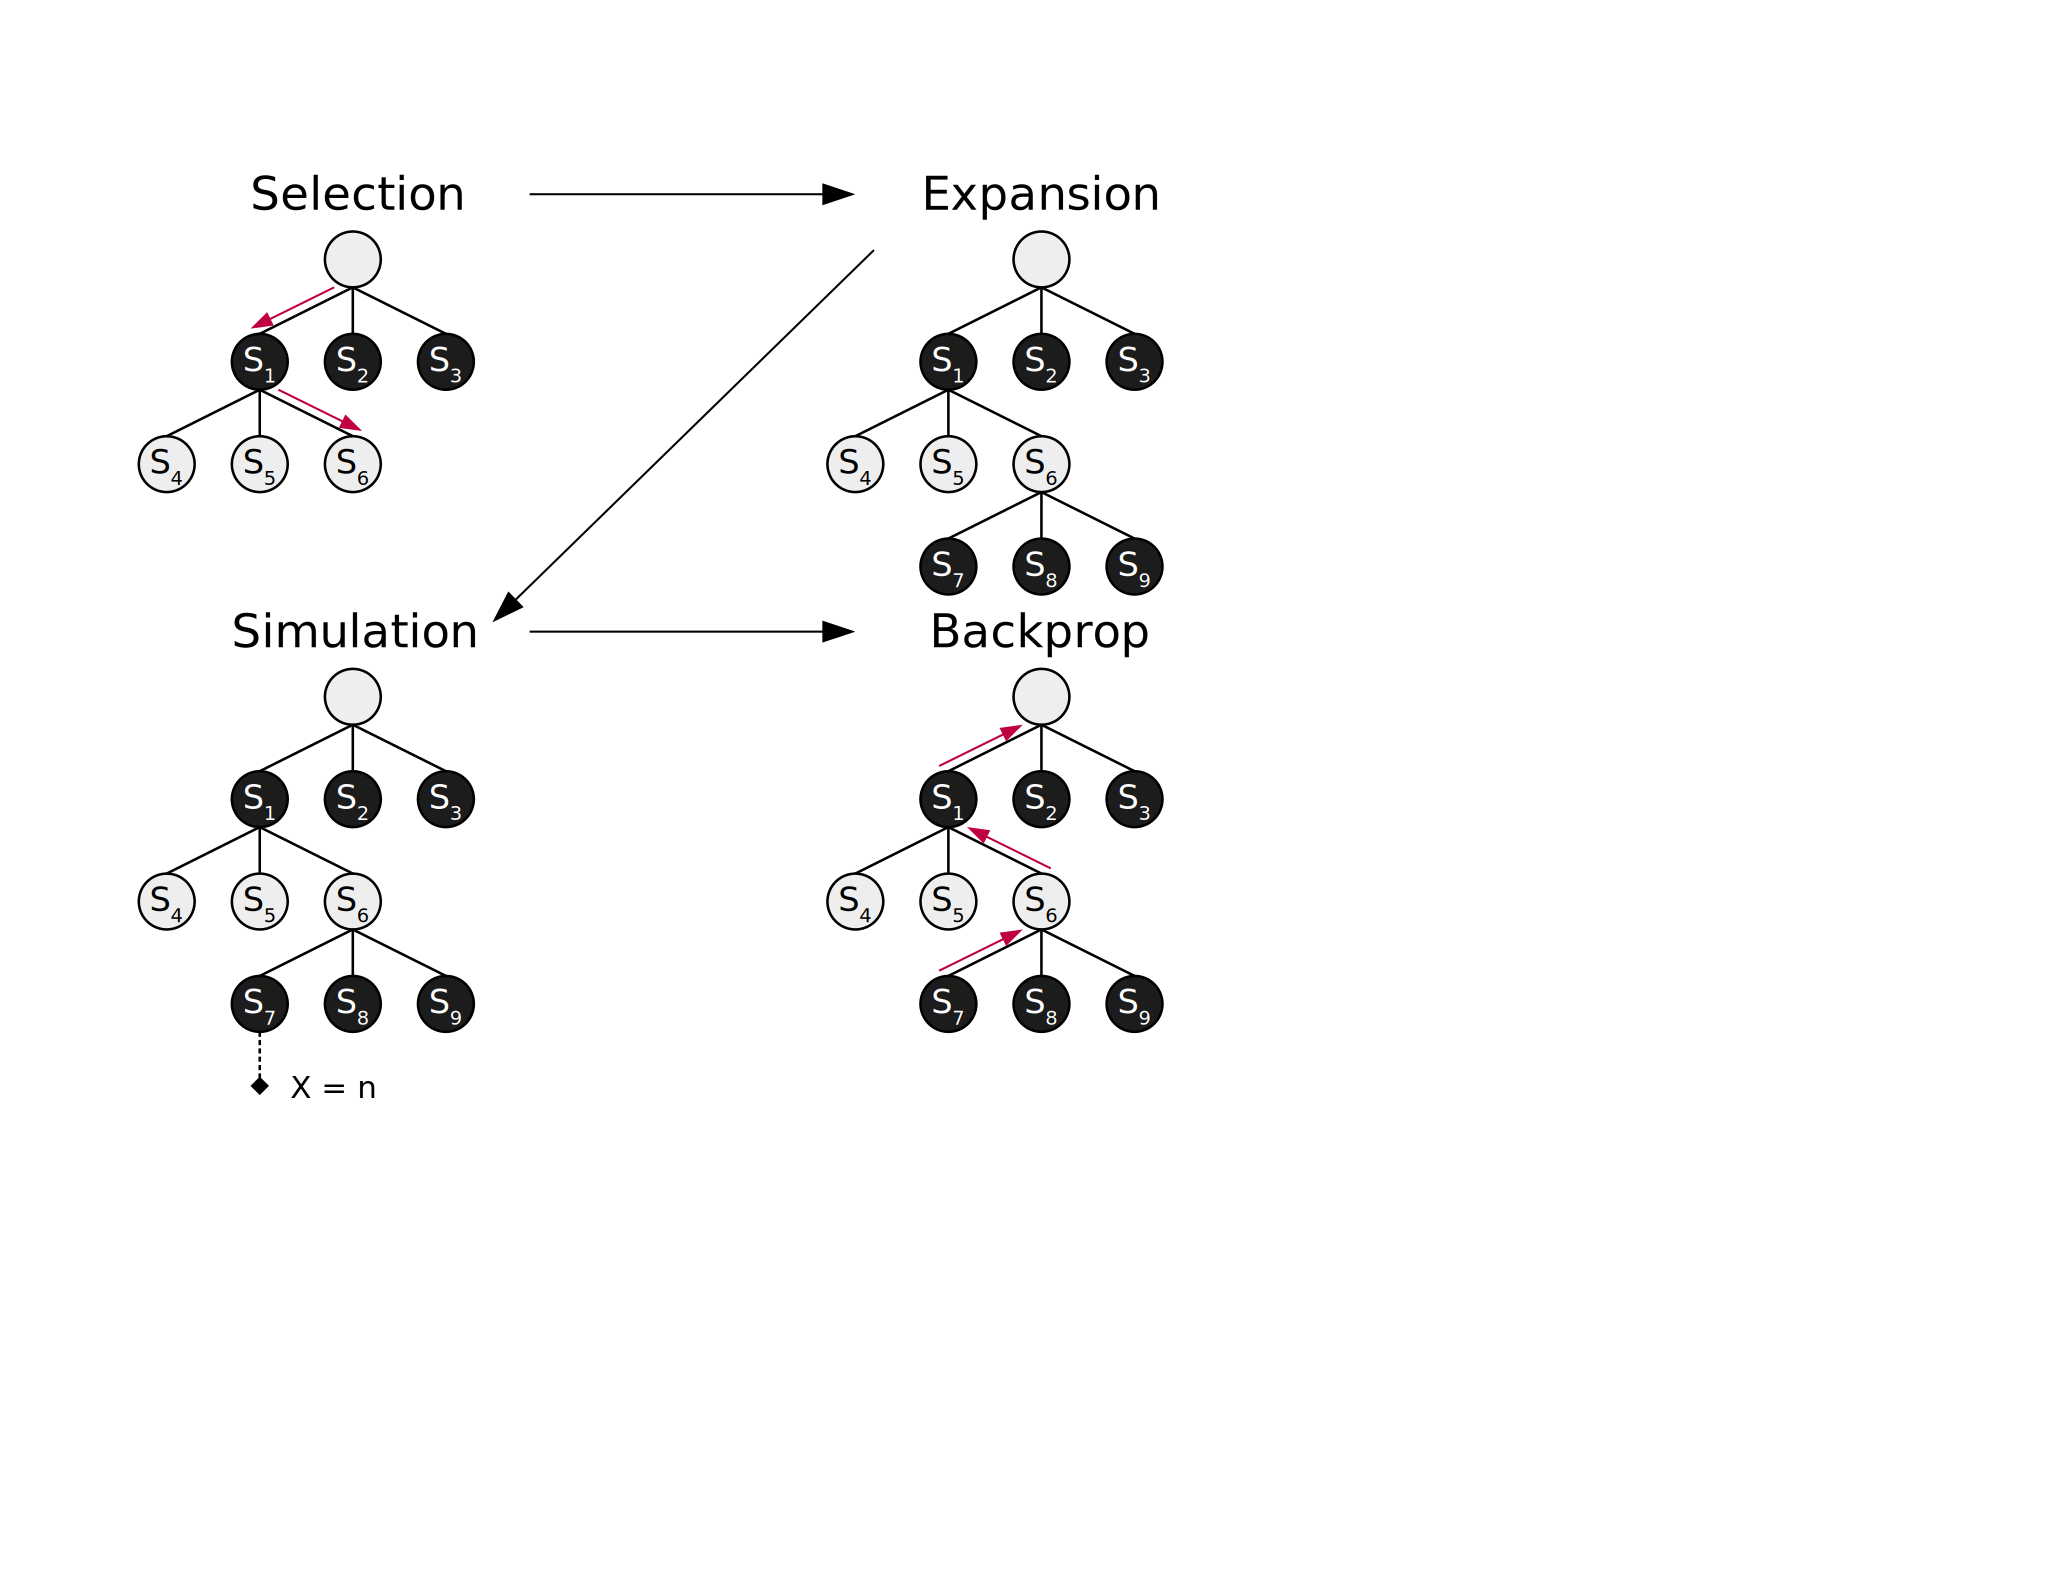
\includegraphics[width=3.5in]{fig/mctsFuncs.png}};
        \node[] at (0.85, 7.5) {\large\circled{1}};
        \node[] at (6.37, 7.5) {\large\circled{2}};
        \node[] at (0.7, 3.92) {\large\circled{3}};
        \node[] at (6.4, 3.92) {\large\circled{4}};
    \end{tikzpicture}
    \caption{4 Main steps for the creation of a Monte Carlo Tree}
    \label{fig:mctsFunc}
\end{figure}

\subsection{Selection}
At the start of each iteration, we initialize at the root of the tree, $id = 0$, and from its children, select the node with the highest associated UCB1 reward:
\begin{equation}
    \label{eq:UCB1}
    \text{UCB1 Node Value: } X + C_p \sqrt{\frac{\ln{n}}{N}}
\end{equation}
\clearpage \noindent with $X$ being the future reward from exploring of the node and its children, $N$ being the number of visits the node has received, and $n$ being the number of visits the parent node has received. The exploration-exploitation parameter, $C_p$, has a value of \(\sfrac{1}{\sqrt{2}}\) which was selected due to its performance demonstrated by Hennes~\cite{Hennes2015}. This reward policy allows the tree to explore all valuable nodes, while still exploiting nodes that return high enough future rewards.

Once a child node has been selected, this process will repeat until a leaf node, one without children, has been reached. As the function navigates down a branch, if, at any point, all of the selected node's children are deemed terminal, such as exceeding the total $\Delta V$ budget, the current node is also declared terminal. When this condition is met, the select function will restart its search process at the root of the tree. With this implementation, the tree is able to further constrict the search space, reducing computation time. Once the selection process leads to a leaf node, the node $id$ will be passed to the next step, the expansion function.

\subsection{Expansion}
When a leaf node is reached and has not been deemed terminal, the next step of the algorithm is to create a new set of state pairs to explore. Before initializing a new group of nodes, we take into account the state of arrival, the child node, and the departure, the parent node. As planetary motion is of conics, Cartesian grid position sampling is not viable. Thus angular divisions are required to efficiently sample a planet's position. For each of the possible planets to visit, the following policy is implemented:
\begin{equation*}
    \label{eq:ephemArray}
    E =
    \left(\begin{array}{c}
        n*(\tau_1 + \tau_0) + t_0 \\
        \vdots \\
        m*(\tau_1 + \tau_0) + t_0 \\
    \end{array}\right)
    \text{ for }
    \left\{\begin{array}{lll}
        n = 0.10, & m = 1.00 &\text{if } a_1 < 2 \text{ AU} \\
        n = 0.05, & m = 0.25 &\text{if } a_1 \geq 2 \text{ AU}
    \end{array}\right.
\end{equation*}

For the ephemeris array $E$, the ephemeris state of the child node is dictated by the period of the node's associated planet, $\tau_1$, and the period of the parent node's planet, $\tau_0$. This array is bounded using the parameters $n$ and $m$, which are defined by the semi-major axis of the child node's planet, $a_1$. The values for $n$ and $m$ for the inner planets, $a_1 < 2$ AU, were selected based upon their performance in Hennes~\cite{Hennes2015}. These values, however, are not ideal for travel to the outer planets. For example, with the previous values, Lambert arc flight times could be in excess of 12 years for a leg to Jupiter. Additionally, if Jupiter is to be used for a gravitational assist to another outer body, faster transfers are required. Based on their performance in simulations, the values of $n = 0.05$ and $m = 0.25$ lead to more transfers that satisfied mission requirements.

With the upper and lower bounds of the array set, an additional parameter for detail, $d$, specifies the length of the array, also defining the resolution of the time steps. Additionally, this allows for dynamic angular detail in the ephemeris arrays. The inner planetary sequences are more sensitive to large time steps which could lead to missed transfers. Thus, the fixed array length leads to smaller time steps for inner planets, and larger for outer planets. For the purpose of this paper, a value of $d = 16$ was found to be sufficient for a majority of calculations as a balance between computation time and detail.

Furthermore, child nodes that revisit the same parent planet have additional ephemeris node tweaks to allow for better performance. The $n$ and $m$ values are set to 0.9, and 1 accordingly, for the set of values in $k$. This allows the tree to search differing, non-impulsive, leveraging orbits of 2:1, 3:1, and 4:1 resonances. At this time, only leveraging sequences with revolutions of less than 1 were allowed. To avoid the singularity solution of the Lambert problem for angles of 0$^\circ$ and 180$^\circ$, the last node is offset by an arbitrary integer number of days. The implementation of Earth specific leveraging orbits is discussed in the next section in greater detail.

\begin{equation*}
    \label{eq:ephemArrayLev}
    E =
    \left(\begin{array}{c}
        k*n*\tau + t_0 \\
        \vdots \\
        k*m*\tau + t_0 - \text{ offset} \\
    \end{array}\right)\hspace{1.5em}
    \text{For } k \text{ in } [2, 3, 4]
\end{equation*}

Once the list of states has been established, a new set of children nodes are created to match all combinations of ephemeris and planetary NAIF ID pairs. In order to further prune the tree to reduce unnecessary calculations, Lambert arcs are calculated to each state pair to evaluate their associated $\Delta V$ cost. Any node that exceeds the mission budget is considered terminal and is not used in any further exploration. To calculate unoptimized mission $\Delta V$ usage, the simulation uses powered flybys, as characterized by Wagner~\cite{Wagner2015}.

The powered flyby geometry consists of an incoming and outgoing spacecraft velocity vectors given by the solutions to the Lambert problem. A graphical overview of this condition is shown in Figure~\ref*{fig:flyby}. This maneuver is used to either bend the trajectory to a desired direction and/or further increase/decrease the magnitude of $V_{\infty-out}$, the relative velocity out of the planet. By manipulating the bend angle and velocity of a gravitational assist, it is possible to patch together two separate Lambert transfers. Therefore, a small $\Delta V$ can be used in order to increase the performance and efficiency of the gravity assists. This $\Delta V$ can be performed at any point along the hyperbolic orbit, but there exists a point of maximum efficiency. Its effectiveness, moreover, is derived from the Oberth effect~\cite{Adams2010}, which states that a $\Delta V$ maneuver is more efficient at changing the overall orbital energy at higher velocities. For this reason, it is common to design the maneuver at periapsis~\cite{Brennan2015}. While this maneuver can be utilized to enhance trajectory characteristics, it serves a different purpose for the tree search, that has the goal of minimizing this value. To mitigate the coarse nature of the search, we use this powered flyby to evaluate the effectiveness of the epoch in which the flyby occurs. For values that exceed the total budget, it can be surmised that the flyby is at a non-optimal time. In addition, while smaller $\Delta V$ flybys lead to ballistic, or near ballistic, solutions, there have been cases where even high $\Delta V$ solutions, $> 1 \text{ } \sfrac{km}{s}$, have been optimized.

\begin{figure}[htb]
    \centering
    \includegraphics[width=2.75in]{fig/flybyGeo.png}
    \setlength{\belowcaptionskip}{-15pt}
    \caption{Geometry of a patch conics flyby with the solid black line being the hyperbolic trajectory, the dotted lines being the asymptotes bounding the conic, $\boldsymbol{\vec{u}_{sun}}$ being axis pointed towards the sun, and $\boldsymbol{\vec{u}_{v}}$ being the vector in the direction of the planet's velocity $\boldsymbol{\vec{V}_{p}}$}
    \label{fig:flyby}
\end{figure}

With the environmental conditions in place, we arrive at the formulation of the boundary value problem (BVP), as described by Wagner\cite{Wagner2015}. It is assumed that the flyby is coplanar, and the plane can be defined by the incoming and outgoing spacecraft velocities and the center of the encounter planet. The conditions that define the BVP are the incoming and outgoing $V_\infty$ and the bend angle, $\delta$. The solution to the BVP is the $\Delta V$ and the value of the maneuver periapsis radius, $r_p$. The first initial condition to the problem is the semi-major axis, $a$, of the incoming and outgoing hyperbolic trajectories, which is defined as:
\begin{equation}
    a_\text{in/out} = -\frac{\mu_p}{v^2_{\infty-\text{in/out}}}
\end{equation}
\noindent where $\mu_p$ is the standard gravitational parameter of the flyby planet. Additionally, the required turn angle from the flyby, $\delta$, is another condition that must be met. This value is found by the following function finding the angle between the incoming and outgoing $V_\infty$ vectors:
\begin{equation}
    \delta = \text{cos}^{-1}\left(\frac{ \vec{\textbf{V}}_{\infty-\text{in}} \cdot \vec{\textbf{V}}_{\infty-\text{out}} }{ V_{\infty-\text{in}} \cdot V_{\infty-\text{out}} }\right)
\end{equation}

With $e_{out}$, the eccentricity of the outbound hyperbolic conic, as the iterated value, a function, and its derivative, can be defined. In order to solve for $e_{out}$, the Newton Raphson root finding method is used to find the eccentricity that coincides with the two $V_\infty$ vectors. For each full loop, an initial $e_{out}$ value of 1.5 is used due to its performance in Wagner \cite{Wagner2015}.

\begin{equation}
    f = \left( \frac{a_{out}}{a_{in}} (e_{out} - 1) \right) \text{sin} \left( \delta - \text{sin}^{-1} \left( \frac{1}{e_{out}} \right) \right)
\end{equation}

\begin{equation}
    \frac{\text{d}f}{\text{d}e_{out}} = \left( \frac{a_{out}}{a_{in}}e_{out} - \frac{a_{out}}{a_{in}} + 1 \right) \frac{ \text{cos}\left( \delta - \text{sin}^{-1} \left( \sfrac{1}{e_{out}} \right) \right) }{ e_{out}^{2} \sqrt{1 - \sfrac{1}{e_{out}^{2}} } } + \frac{a_{out}}{a_{in}}\text{cos}\left( \delta - \text{sin}^{-1} \left( \sfrac{1}{e_{out}} \right) \right)
\end{equation}

Once a value of $e_{out}$ has been found, it can then be used to find the actual periapsis radius, which is then used to find the required maneuver $\Delta V$. In addition, the periapsis radius is checked against a set minimum flyby altitude.

\begin{equation}
    r_p = a_{out}(1 - e_{out})
\end{equation}

\begin{equation}
    \Delta V_{GA} = \left| \sqrt{ v^2_{\infty-\text{in}} + \frac{2\mu_p}{r_p} } - \sqrt{ v^2_{\infty-\text{out}} + \frac{2\mu_p}{r_p} } \right|
\end{equation}

While this results in an increased computation cost at each step of the node creation process, this method of $\Delta V$ calculation allows for a better approximation of actual trajectory performance. In addition to powered flyby $\Delta V$'s, budget usage was also calculated for launch energies higher than the specified limit. If, for example, the max launch energy was defined as $V_\infty = 6 \text{ }\sfrac{km}{s}$ and the spacecraft launched at a $V_\infty$ = 7 $\sfrac{km}{s}$, the incurred $\Delta V$ cost would be 1 $\sfrac{km}{s}$. After the states have been created, and the nodes pruned, the expand function selects the new node with the lowest associated $\Delta V$ cost to continue onto the simulation step.

\subsection{Simulation}

On the tree's arrival to an unvisited leaf node, the node's future expected reward, $X$, must be calculated. A group of temporary state pairs is expanded from the leaf, as the starting point for the random exploration. For each new node, the program will randomly walk through additional state pairs, generated in the same fashion as in the expand function, calculating the $\Delta V$ in the process, until a termination state is reached. When either the budget is expended, or the target planet is reached, the associated cost is calculated using the following equation:

\begin{equation}
    \label{eq:simCost1}
    X = \text{max}\left( 0.1 \cdot l,\hspace{0.5em} \frac{\Delta V_{budget} - \Delta V_{used}}{\Delta V_{budget}} \right)
\end{equation}

Upon termination, we balance the reward between two criteria: $\Delta V$ usage and the number of flybys completed, $l$. If the final destination is not reached within the allowed budget, the algorithm will still provide a small bonus to a simulation completing Lambert arcs. After all temporary states have been simulated, the reward returned from each is averaged and output from the function to be passed back up the branch in the backpropagation step.

\subsection{Backpropagation}

At the end of the core MCTS loop, the backpropagation step communicates the expected reward from a leaf node back up the branch to reflect a more accurate reward of a branch. Eq. \eqref{eq:bp} is used to calculate the new reward, where $X$ is the current reward value at each node. This value is then adjusted by a weighted average based on the number of current visits, $N$, to each node of the branch.

\begin{equation}
    \label{eq:bp}
    X_{node, new} = \frac{X_{node, old} \cdot N_{node} + X_{new}}{N_{node} + 1}
\end{equation}

Once the cost is propagated up the tree, the loop restarts at another iteration, exploring a new set of state pairs. This process will repeat until the computation budget is depleted. At completion, the tree will evaluate all leaf nodes that meet the mission constraints to pass to the next step in the trajectory design process, optimization.

\section*{$\boldsymbol{\Delta V}$EGA Maneuver Implementation}
\pdfbookmark[1]{dVEGA Maneuver Implementation}{dv}

A $\Delta V$EGA orbit, also referred to as a leveraging orbit specifically of Earth, launches with the intent to use a gravity assist from Earth for a higher post-flyby heliocentric energy\cite{Hollenbeck}. Leveraging orbits are classified by their nominal resonance period multiple with respect to the flyby body's heliocentric orbit, and we will refer to this number as "$k$". For example, a leveraging orbit that has a period roughly 3 times as large as Earth's will have a $k=3$ which is represented as a 3:1 $\Delta V$EGA trajectory. The actual period of these orbits will vary either greater than or less than the nominal time due to encountering the body at a different Earth heliocentric true anomaly. Trajectories with a larger period are referred to as $k$:$1^{+} \Delta V$EGA and those with a shorter are $k$:$1^{-} \Delta V$EGA trajectories. To modify the Earth flyby true anomaly a maneuver at the aphelion, referred to as a deep space maneuver, is executed.

The deep space maneuver (DSM) and subsequent Earth launch characteristics are calculated before the tree generation in order to reduce the number of computations within the search. We approximate the launch $V_\infty$ and DSM $\Delta V$ requirements. The inclusion of the DSM and intercept Earth encounter location reduces the discontinuous trajectory endpoint velocities needed to patch Earth-Earth flyby sequences. Having the required aphelion $\Delta V$ can also aid the optimization process initial guess. A lookup table sorted by the nominal resonance multiple, $k$, and encounter true anomalies, $\theta_{E}$, contains the resulting leveraging orbit properties and maneuver magnitudes. As a low-fidelity approximation, a circular Earth orbit and coplanar trajectories assumptions are used. Finding the $\Delta V$EGA orbit parameters for a specific $\theta_{E}$ and $k$ begins with assuming a nominal orbit period launch and its associated $V_\infty$. The state elements are computed at Earth and the resulting aphelion radius and velocity are found. Because the intercept true-anomaly is fixed, its location and the time it takes to reach the point are known. Eq.~\eqref{eq:dteqn} is the difference in time from the DSM maneuver location to the Earth gravity assist (EGA) point, where $\tau_E$ is the orbital period of Earth.

\begin{equation}
	\label{eq:dteqn}
	dt = k\tau_E \pm \tau_E(\theta_E/2\pi)
\end{equation}

\begin{figure}[htb]
	\centering\includegraphics[width=3.6in]{./fig/dsmmatlab}
    \caption{Example of a computed 3:$\boldsymbol{1^- \Delta V}$EGA trajectory with a final aphelion radius roughly that of Saturn's semi-major axis. The launch $\boldsymbol{V_\infty}$ is 6.97 km/s and the required DSM $\boldsymbol{\Delta V}$ is 0.39 km/s. The EGA flyby altitude was constrained to 200 km, which yielded the highest post flyby energy.}
	\label{fig:dsmmatlab}
\end{figure}

A Lambert arc is computed between these points and the resulting initial velocity change is used to find the DSM vector. The final velocity vector is assumed to be the heliocentric velocity of the leveraging orbit at the EGA. The relative velocity, $\vec{\textbf{V}}_{\infty}$, is computed and a planar flyby of Earth can now be calculated from the tree search algorithm. Figure~\ref{fig:dsmmatlab} illustrates an example leveraging orbit being calculated for $\theta_{E}$ = 40.$7^{\circ}$. An energy maximizing flyby and propagation to the new aphelion is added to the end of the $\Delta V$EGA orbit to show the resulting trajectory.

From testing, we noticed that as $\mid\theta_E\mid$ increased, a normal component in the orbit plane of the DSM $\Delta V$ appeared and grew larger. To limit the $\Delta V$ to only a tangential component, and in return to reduce the total $\Delta V$ required, a minimizer is employed. This optimization comes at the expense of higher launch energy and longer flight time for trajectories requiring large $\mid\theta_E\mid$. Differing trends from Sims et al. analysis of $V_\infty$ leveraging\cite{sims1994} were only noticed in high total $\Delta V$ cases for each $k$ leveraging orbit family. These solutions were discarded from the lookup table due to delivering lower aphelion radii post-flyby when compared to lower total $\Delta V$ leveraging orbits of the same family. The case presented in Figure~\ref{fig:dsmmatlab} is intended to match that discussed by Sims et al\cite{Sims1997} and has nearly identical results. The inclusion of deep space maneuvers, not specific to $\Delta V$EGAs, are not implemented in the current form of the tree search. However, because the algorithm patches the two conics forming the leveraging orbit using Lambert's method, the possibility to extend DSM maneuvers for off-tangent $V_\infty$ departures and targeting for the flyby can be implemented. This inclusion adds another dimension to the lookup table, but offers greater flexibility in the placement of  leveraging maneuvers in the sequence. It can also include $V_\infty$ leveraging of other planets.

Now that the $\Delta V$EGA orbit properties are known, the lookup table solution can be extended to the actual solar system model in the tree search. The table values are represented in a rotating relative frame with respect to Earth's state vector at the launch epoch. A subsequent transformation of the departure velocity and pre-EGA incoming $\vec{\textbf{V}}_{\infty}$ can be done in order to find their specific components corresponding to an Earth epoch in the Ecliptic J2000 frame. From the initial node in the tree, a set of Earth leveraging state pair nodes are created corresponding to their respective $k$ and $\theta_E$ parameters. The number of these leveraging nodes included in the tree is directly related to the angular spacing of $\theta_E$. If the resolution becomes finer by increasing the $\textit{detail}$ input, $d$, the estimated $\Delta V$ becomes more accurate. This, however, increases of the number of tree nodes created, and so for an estimation of the trajectory search space, a coarse resolution is preferred. The discontinuous $\Delta V$ post-EGA required to patch the incoming leg from the leveraging orbit and outgoing leg to the next planet node will determine if the leveraging node and its performance is effective for the transfer. Using this method, a distinction between the $\Delta V$EGA trajectory families to different outer planets can be observed.

\section*{Performance Evaluation}
\pdfbookmark[1]{Performance Evaluation}{cases}

To validate the methods presented in this paper, multiple case studies were tested and evaluated. Three major cases were explored to highlight the different core functionalities of the algorithm. The first case is a search to find Europa Clipper's EELV~\cite{Buffington2014} trajectory involving a sequence of four planetary flybys to test MCTS's ability to find long sequence trajectories. The second study is designed to test the limits of powered flyby $\Delta V$ theory, by finding Galileo's low budget trajectory to Jupiter with similar efficiency. The final case is not based on any historical mission, but evaluates the $\Delta V$EGA theory by finding a variety of the launch possibilities for a Trident-like mission to Neptune.

In addition to roughly matching existing trajectories, search results will be used as initial conditions for an optimization program, MALTO (Mission Analysis Low Thrust Optimizer), to validate the tree search's astrodynamics. While this software is primarily built for low-thrust applications, the program is capable of optimizing for ballistic and chemical propulsion trajectories~\cite{Sims2006}. For each leg of the mission, the optimizer was allowed $\pm$ 100 days, unless otherwise stated, on either side of the tree search's initial guess to mitigate the coarse nature of the broad search constraints.

\subsection{Case 1: Europa Clipper Trajectory Recreation}

The first case is a search to find a sequence similar to Europa Clipper's interplanetary trajectory (15F9-A22 EEVEEJ) utilizing multiple gravitational assists of Earth and Venus to reach Jupiter \cite{Buffington2014}. The nominal trajectory has the spacecraft set to launch on June 03, 2022, and arriving at Jupiter on January 15, 2030, with a three Earth flybys and a Venus flyby. The primary challenge for this mission is the complexity of the sequence, as the difficulty of the combinational problem grows non-linearly with length.

\begin{table}[htb]
    \centering
    \caption{Constrain Input Table for Europa Clipper Trajectory Search}
    \label{table:clipInputs}
    \begin{tabular}{lc}
        \toprule
        \textbf{Input} & \textbf{Value}\\
        \midrule
        Arrival Planet & Jupiter \\
        Launch Window \hspace{1em}& March 01 --- September 01, 2022 \\
        Iterations & 75,000 \\
        $\Delta V$ Budget & 10 $km/s$ \\
        Max C3 & 10 $km^2/s^2$ \\
        Detail ($d$) & 24 \\
        \bottomrule
    \end{tabular}
\end{table}

Table~\ref*{table:clipInputs} provides the search criteria for the Monte Carlo Tree Search. For general trajectory searches, an iteration budget of 50,000 was found to be sufficient, but due to the length of the planetary sequence for the nominal trajectory, we adjusted the limit. Runs with a $d = 16$, the ephemeris array length, were also conducted, but due to the coarseness in the separation of state pairs, the exact solution was deemed infeasible. As described earlier, this behavior is one of the drawbacks of grid searches as not all possible solutions can be found.

At the completion of the search, 20 million Lambert arcs had been conducted, and a tree of one million tree nodes was created. Of the 1.9 billion combinations possible for a six-layer tree, only 275 solutions were deemed feasible for the input criteria. Figure~\ref*{fig:clipResults} (Left) shows the top 100 trajectories, sorted by their unoptimized mission $\Delta V$ with the nominal solution circled and shown on the (Right). The targeted sequence was the ninth highest result in terms of unoptimized $\Delta V$ usage behind an EEVVEJ and EEVEJ sequence. The trajectory's low placement is down to the final Earth flyby, which, even under ideal conditions, requires an unoptimized flyby $\Delta V$ of 3.23 $\sfrac{km}{s}$. Among all top trajectories, the initial two flybys of Earth and Venus were found to share similar dates. Of the EEVEEJ solutions found, the most optimal utilized a 3:1 orbital resonance for the final Earth flyby, while the nominal trajectory utilized a 2:1. The 2:1 solutions also exist within the results, but do not appear until later is the data set, utilizing an additional 250 $\sfrac{m}{s}$ of $\Delta V$. Even with this deviation, to a 3:1 orbit, the Jupiter arrival occurred only one month later than targeted and has a lower $V_{\infty-in}$.
\begin{figure}[!ht]
    \centering
    \begin{subfigure}
        \centering\includegraphics[width=2.4in]{./fig/clipperResults.png}
    \end{subfigure}
    \begin{subfigure}
        \centering
        \begin{tikzpicture}
            \node[anchor=south west,inner sep=0] (image) at (0,0) {\includegraphics[width=2.5in]{./fig/clipperMCTS.png}};
        \end{tikzpicture}
    \end{subfigure}
    \setlength{\belowcaptionskip}{-10pt}
    \caption{(Left) Top 100 results from the broad search colored by sequence\hspace{1em} (Right) Circled, unoptimized trajectory from results that matches targeted sequence \cite{Buffington2014} with the outermost dashed line is the semi-major axis of Jupiter, the middle dashed line is Earth's, and the innermost is Venus's.}
    \label{fig:clipResults}
\end{figure}

The encounter dates from the best performing EEVEEJ transfer was used for optimization. Table~\ref*{table:clipMInputs} shows initial guess supplied to the optimizer by MCTS as well as the post optimized dates returned. To reduce the $V_{\infty-in}$ at Jupiter, the node's date bounds were adjusted to be $\pm$ 500 days. Figure \ref*{fig:clipMalto} shows the optimized trajectory. The resulting trajectory was well within the bounds placed on the optimizer for the flybys and arrival dates. As well, due to the increased arrival bounds, the $V_\infty$ into Jupiter was reduced. In addition, the largest departure from the initial guess dates, apart from Jupiter arrival, was the third flyby of Earth. The date had transitioned 1.5 months later than initially chosen, leading to an orbit of more than one complete revolution. With this test complete, it's seen that the Monte Carlo Tree Search algorithm is capable of searching out long sequence interplanetary trajectories that need minimal tweaking in the optimization process.
\begin{table}[htb]
    \begin{center}
        \caption{MCTS output dates vs optimized dates for Europa Clipper}
        \label{table:clipMInputs}
        \begin{tabular}{lcc}
            \toprule
            \multirow{2}{*}{\textbf{Planetary Node}} & \multicolumn{2}{c}{\textbf{Dates}}\\
            \cmidrule{2-3}
            {} & \textbf{MCTS} & \textbf{Optimized}\\
            \midrule
            Launch          & June 04, 2022     & May 12, 2022 \\
            Earth Flyby \#1 & June 02, 2023     & May 12, 2023 \\
            Venus Flyby     & November 23, 2023 & November 22, 2023 \\
            Earth Flyby \#2 & October 22, 2024  & October 2, 2024 \\
            Earth Flyby \#3 & October 20, 2027  & December 2, 2027 \\
            Jupiter Arrival & February 13, 2030 & March 17, 2031 \\
            \bottomrule
        \end{tabular}
    \end{center}
\end{table}
\begin{figure}[h!tb]
    \centering
    \begin{tikzpicture}
        \node[anchor=south west,inner sep=0] (image) at (0,0) {\includegraphics[width = 5in]{./fig/clipperMalto.png}};
        % NUMBER 1
        \node[] at (9.75, 8.5) {\large\circled{1}};
        \node[] at (4.45, 6.55) {\large\circled{1}};
        % NUMBER 2
        \node[] at (9.75, 7.25) {\large\circled{2}};
        \node[] at (4.75, 6.15) {\large\circled{2}};
        % NUMBER 3
        \node[] at (9.75, 5.1) {\large\circled{3}};
        \node[] at (5.2, 7.8) {\large\circled{3}};
        % NUMBER 4
        \node[] at (9.75, 3) {\large\circled{4}};
        \node[] at (7.2, 7.8) {\large\circled{4}};
        % NUMBER 5
        \node[] at (7.2, 3) {\large\circled{5}};
        \node[] at (6.5, 8.6) {\large\circled{5}};
        % NUMBER 6
        \node[] at (4.75, 2.9) {\large\circled{6}};
        \node[] at (4.45, 1.8) {\large\circled{6}};
    \end{tikzpicture}
    \setlength{\belowcaptionskip}{-10pt}
    \caption{Optimized Europa Clipper trajectory from tree search results}
    \label{fig:clipMalto}
\end{figure}
\subsection{Case 2: Galileo Trajectory Recreation}

For the second validation case, the nominal trajectory of Galileo has the spacecraft set to launch from Earth with a C3 of 13--17 $\sfrac{km^2}{s^2}$ on October 18, 1989, and arriving at Jupiter on December 07, 1995, with a Venus flyby and an Earth 2:1 resonance sequence. The major challenge behind this sequence was for the algorithm to be able to find the low required $\Delta V$ solution as described by D'Amario~\cite{DAmario1992}. For Galileo's interplanetary leg of its trajectory design, the spacecraft was only budgeted 100 $\sfrac{m}{s} \text{ of } \Delta V$ for TCMs, trajectory correction maneuvers.

\begin{table}[htb]
    \centering
    \caption{Constrain Input Table for Galileo Trajectory Search}
    \label{table:galiInputs}
    \begin{tabular}{lc}
        \toprule
        \textbf{Input} & \textbf{Value}\\
        \midrule
        Arrival Planet & Jupiter \\
        Launch Window & Jun 01 --- Dec 31, 1989 \\
        Iterations & 50,000 \\
        $\Delta V$ Budget & 3 $\sfrac{km}{s}$ \\
        Max Arrival $V_{\infty}$ & 7.5 $\sfrac{km}{s}$  \\
        Max C3 & 20 $\sfrac{km^2}{s^2}$ \\
        Detail ($d$) & 16 \\
        \bottomrule
    \end{tabular}
\end{table}

Table~\ref*{table:galiInputs} lays out the inputs to the search algorithm, which fall more in line with the average use case. In order to constrain the results to the low $\Delta V$ solution, the $\Delta V$ budget was set to 3 $\sfrac{km}{s}$, and the maximum C3 was rounded to a value of 20 $\sfrac{km^2}{s^2}$. An additional constraint was placed on the search, requiring a low energy arrival to Jupiter, to further prune the results. As a silent constraint for all searches, solutions will also be required to have a radially $V_\infty$ greater than -3 $\sfrac{km}{s}$ or less than +3 $\sfrac{km}{s}$ for radial in and out arrivals accordingly. This was implemented so that solutions contained the correct arrival $V_\infty$ direction, and value were found.

\begin{figure}[htb]
    \begin{subfigure}
        \centering\includegraphics[width=2.75in]{./fig/galileoResults.png}
    \end{subfigure}
    \begin{subfigure}
        \centering
        \begin{tikzpicture}
            \node[anchor=south west,inner sep=0] (image) at (0,0) {\includegraphics[width=3in]{./fig/galileoMCTS.png}};
            % \node[] (text) at (2, 6.3) {\scriptsize Jupiter SMA};
        \end{tikzpicture}
    \end{subfigure}
    \caption{(Left) Top results from built broad search colored by sequence\hspace{1em} (Right) Circled, unoptimized trajectory from results that matches targeted sequence \cite{DAmario1992} with the outermost dashed line is the semi-major axis of Jupiter, the middle dashed line is Earth's, and the innermost is Venus's.}
    \label{fig:galiResults}
\end{figure}

The tree made 867,000 nodes and conducted 10 million Lambert arcs, in order to find the 12 solutions to the constraints. Of those solutions, the eighth was the nominal targeted trajectory. Figure \ref*{fig:galiResults} (Left) shows the 12 solutions ranked by their unoptimized mission $\Delta V$ usage, and the (Right) shows the circled nominal trajectory. In the same fashion as the Europa Clipper case, the optimal found trajectory deviates from what Galileo originally performed. The final Earth flyby was conducted in a 3:1 resonance rather than a 2:1 resonance and led to an overall smaller incoming $V_\infty$. The 2:1 resonance case also exists within the found data set, but is the 11 of 12 that satisfies the criteria. Similar to Europa Clipper, with the additional one year resonance, the spacecraft only arrives at Jupiter 3 months after targeted. With the trajectory leg dates, this solution will be optimized using MALTO to find the optimized version of this trajectory.
\begin{table}[htb]
    \begin{center}
        \caption{MCTS output dates vs optimized dates for Galileo}
        \label{table:galiMInputs}
        \begin{tabular}{lcc}
            \toprule
            \multirow{2}{*}{\textbf{Planetary Node}} & \multicolumn{2}{c}{\textbf{Dates}}\\
            \cmidrule{2-3}
            {} & \textbf{MCTS} & \textbf{Optimized}\\
            \midrule
            Launch          & October 21, 1989  & October 06, 1989\\
            Venus Flyby     & February 27, 1990 & February 14, 1990 \\
            Earth Flyby \#1 & December 29, 1990 & December 15, 1990 \\
            Earth Flyby \#2 & December 26, 1993 & December 14, 1992 \\
            Jupiter Arrival & March 03, 1996    & June 24, 1996 \\
            \bottomrule
        \end{tabular}
    \end{center}
\end{table}

\begin{figure}[htb]
    \centering
    \begin{tikzpicture}
        \node[anchor=south west,inner sep=0] (image) at (0,0) {\includegraphics[width=5in]{./fig/galileoMalto.png}};
        % NUMBER 1
        \node[] at (9.75, 8.5) {\large\circled{1}};
        \node[] at (7, 6.8) {\large\circled{1}};
        % NUMBER 2
        \node[] at (9.75, 7.25) {\large\circled{2}};
        \node[] at (5.85, 7.35) {\large\circled{2}};
        % NUMBER 3
        \node[] at (9.75, 5.1) {\large\circled{3}};
        \node[] at (6.05, 8.3) {\large\circled{3}};
        % NUMBER 4
        \node[] at (9.85, 3) {\large\circled{4}};
        \node[] at (6.55, 8.3) {\large\circled{4}};
        % NUMBER 5
        \node[] at (7.4, 2.4) {\large\circled{5}};
    \end{tikzpicture}
    \caption{Optimized Galileo trajectory from tree search results}
    \label{fig:galiMalto}
\end{figure}
\clearpage
When inputting trajectory dates into the optimizer, it was found the 3:1 sequence suggested was not as viable compared to other options. When converging the trajectory, it was found that the performance of the 3:1 trajectory was too high for the spacecraft to properly capture at Jupiter. Thus by increasing the bounds of the final Earth flyby to bounds of $\pm$500 days to give more leeway, the optimizer converged on a solution that utilized a 2:1 orbit as opposed to the 3:1. This result can be found in Figure \ref*{fig:galiMalto}. This result aligns with the findings by Sims \cite{sims1994} where 3:1 orbits were capable of reaching aphelion heights of Uranus SMA, while 2:1 trajectories can reach aphelion heights of 8 AU. Doing so allowed the work of the Jupiter transfer to be shared between the two Earth flybys without exceeding their energy capacities. As in Table \ref*{table:galiMInputs}, even after taking a year off the total flight time to the last Earth flyby, the Jupiter arrival was only set back 113 days.
\subsection*{Case 3: Triton $\boldsymbol{\Delta V}$EGA Opportunity Search}
\pdfbookmark[2]{Case 3: Triton dVEGA Opportunity Search}{triton}

Now that the sequencing ability of the tree search algorithm has been verified, we can now extend its use to an exploratory context. With interest in exploring the solar system's icy moons, a sequence to Neptune, and in turn Triton, is explored\cite{Hubbard2010}. An arbitrary launch period was selected for this evaluation, and the search is limited to trajectories with the inclusion of a $\Delta V$EGA to evaluate its integration and performance. The number of iterations was set at 15,000 as this search has a maximum depth of 4 nodes, greatly reducing the size of the tree. To achieve fast transfer times to Neptune, the use of Jupiter for gravitational assists is critical, as the energy Jupiter can add to a heliocentric orbit is significantly more efficient than any direct launch, in terms of $\Delta V$ usage \cite{Landau2010}. Additionally, it is desired to have a higher incoming relative velocity at Jupiter in order to have the appropriate outgoing energy to reach Neptune. With this in mind, the intent of the search was to find $\Delta V$EGA trajectories that deliver a high post-EGA semi-major axis so the encounter velocity is maximized. The $\textit{detail}$ is set to 16 which creates 8 $k$:1$^{-}$ and 8 $k$:1$^{+}$ nodes for each $k$ family. This spread is a balanced compromise between computation time, due to the number of nodes created, and the accuracy of the DSM's $\Delta V$ estimate. The launch C3 is set to 60 $km^2/s^2$ to allow the tree to mainly explore 2:1 and 3:1 $\Delta V$EGAs with the possibility of 4:1 leveraging families, at an additional $\Delta V$ cost. The results of the input search space are summarized in Table~\ref{tab:tritonInputs}:

\begin{table}[htb]
    \begin{center}
        \caption{Inputs for $\boldsymbol{\Delta V}$EGA Trajectories to Neptune via Jupiter}
        \label{tab:tritonInputs}
        \begin{tabular}{lc}
            \toprule
            \textbf{Input Name} & \textbf{Input Value}\\
            \hline
            Arrival Planet & Neptune \\
            Launch Window \quad \quad & Jan 01, 2029 --- Jan 01, 2030 \\
            Iterations & 15,000 \\
            $\Delta V$ Budget & 3 $\sfrac{km}{s}$ \\
            Max C3 & 60 $\sfrac{km^2}{s^2}$ \\
            Detail ($d$) & 16 \\
            \bottomrule
        \end{tabular}
    \end{center}
\end{table}
\begin{figure}[htb]
    \centering
    \begin{tikzpicture}
        \node[anchor=south west,inner sep=0] (image) at (0,0) {\includegraphics[width=3.6in]{./fig/tridentMCTS}};
    \end{tikzpicture}
    \setlength{\belowcaptionskip}{-10pt}
	\caption{Different resulting E($\boldsymbol{$k$:$1$^{+/-}}$)EJN sequence types from the search. The outermost dashed line is the semi-major axis of Jupiter, the middle dashed line is Earth's, and the innermost is Venus's. The $\boldsymbol{\Delta V}$EGA type is labeled above and the mark on the leveraging orbit denotes the approximate DSM location.}
	\label{fig:tridentMCTS}
\end{figure}

The search completed and resulted in 65 sequences from the 704,000 nodes created and 7 million Lambert arcs performed. As expected, most solutions used the 2:1 or 3:1 leveraging maneuvers, and a few 4:1 sequences were also found, but with larger unoptimized $\Delta V$ values. Figure~\ref{fig:tridentMCTS} shows the four different $\Delta V$EGA sequence types that comprise a majority of the search results. As a general trend, the 3:1 solutions yielded higher energy transfers to Jupiter and allowed them to achieve faster transfer times onto Neptune.

Optimizations of select tree search solutions are conducted to determine the accuracy of the sequences found and to further investigate the deep-space maneuver performance. The 2:1 and 3:1 $\Delta V$EGA trajectories are of interest as these families are able to reach Jupiter with favorable flight times, launch energies, and incoming relative velocities. The flight time and encounter epochs from the tree search are compared to the optimized solution to better understand the performance and limitations of the search algorithm. For the optimization process, all initial guess conditions were taken from the tree search output and the following bounds were set for encounter epochs. For Earth encounters and the DSM epoch, a $\pm$30-day span is used to keep the sequence relatively similar to the tree search conditions. For the Jupiter and Neptune flybys, 50 and 300 days are used respectively. This looser date bound accounts for the larger spacing in epochs for the outer planets' nodes in the tree. The maximum launch $V_\infty$ is allowed to be 0.1 $km/s$ over the predicted requirement from the search, and the limits on the DSM $\Delta V$ are $\pm$0.4 $km/s$ from the estimated value from the lookup table solution. Figure~\ref{fig:maltotriton} shows examples of two optimized trajectories resulting from the search. The left plot is an example of a 2:1$^{+}$ $\Delta V$EGA which requires a launch $V_\infty$ magnitude of 5.20 $km/s$ (as opposed to the \hspace{0.5px} 5.15 $km/s$ from the prediction). The 2:1 leveraging trajectory has an incoming $V_\infty$ to Jupiter of around 9 $km/s$ which yields a 4900 day (13.4 years) flight time to Neptune. This case utilized an intercept $\theta_E$ of 42$^\circ$ which has an estimated DSM $\Delta V$ of 0.43 $km/s$, while the optimizer's computed 0.66 $km/s$. The right plot from Figure~\ref{fig:maltotriton} shows a 3:1$^{-}$ trajectory with an Earth departure $V_\infty$ of 6.98 $km/s$ and a DSM $\Delta V$ of 0.41 $km/s$. The estimated performance from the tree search is 6.97 $km/s$ and 0.40 $km/s$ for the launch relative velocity and DSM respectively. The similarities between the tree results and the optimized cases presented indicate that the search algorithm is generally able to produce useful initial guesses for the optimization process.
\clearpage
\begin{table}[htb]
    \centering
    \centering
    \caption{MCTS output dates vs optimized dates for $\boldsymbol{\Delta V}$EGA missions to Neptune}
    \label{table:tridMInputs}
    \begin{tabular}{lcc|cc}
        \toprule
        \multirow{2}{*}{\textbf{Planetary Node}} & \multicolumn{2}{c}{$\boldsymbol{2:1^+}$} & \multicolumn{2}{c}{$\boldsymbol{3:1^-}$}\\
        \cmidrule{2-3} \cmidrule{4-5}
        {} & \textbf{MCTS} & \textbf{Optimized} & \textbf{MCTS} & \textbf{Optimized}\\
        \midrule
        Launch            & Jan 01, 2029 & Jan 11, 2029 & May 01, 2029 & Apr 28, 2029 \\
        Earth Flyby       & Mar 07, 2031 & Mar 05, 2031 & Mar 07, 2032 & Mar 20, 2032 \\
        Jupiter Flyby \#1 & Jan 08, 2033 & Nov 16, 2032 & Jul 25, 2033 & Aug 14, 2033 \\
        Neptune Arrival   & Jun 26, 2042 & Jun 12, 2042 & May 06, 2042 & Aug 13, 2042 \\
        \bottomrule
    \end{tabular}
\end{table}
\begin{figure}[htb]
    \centering
    \begin{subfigure}
        \centering
        \begin{tikzpicture}
            \node[anchor=south west,inner sep=0] (image) at (0,0) {\includegraphics[width=2.9in]{./fig/eejn21plus}};
            % NUMBER 1
            \node[] at (3, 4.9) {\scriptsize\circled{1}};
            \node[] at (1.33, 5) {\scriptsize\circled{1}};
            % NUMBER 2
            \node[] at (1.35, 1.55) {\scriptsize\circled{2}};
            \node[] at (2.5, 3.0) {\scriptsize\circled{2}};
            % % NUMBER 3
            \node[] at (0.8, 3) {\scriptsize\circled{3}};
            \node[] at (0.85, 4.4) {\scriptsize\circled{3}};
            % % NUMBER 4
            \node[] at (3.3, 2.6) {\scriptsize\circled{4}};
            \node[] at (4.3, 1) {\scriptsize\circled{4}};
            % % NUMBER 5
            \node[] at (5.7, 4.15) {\scriptsize\circled{5}};
        \end{tikzpicture}
    \end{subfigure}
    \begin{subfigure}
        \centering
        \begin{tikzpicture}
            \node[anchor=south west,inner sep=0] (image) at (0,0) {\includegraphics[width=2.9in]{./fig/eejn31minus4850}};
            % NUMBER 1
            \node[] at (0.9, 1.95) {\scriptsize\circled{1}};
            \node[] at (1.25, 2.85) {\scriptsize\circled{1}};
            % NUMBER 2
            \node[] at (3.5, 5) {\scriptsize\circled{2}};
            \node[] at (3.15, 4.5) {\scriptsize\circled{2}};
            % % NUMBER 3
            \node[] at (1.6, 4.5) {\scriptsize\circled{3}};
            \node[] at (1.15, 3.2) {\scriptsize\circled{3}};
            % % NUMBER 4
            \node[] at (3.8, 2.7) {\scriptsize\circled{4}};
            \node[] at (5, 1.05) {\scriptsize\circled{4}};
            % % NUMBER 5
            \node[] at (5.7, 3.9) {\scriptsize\circled{5}};
        \end{tikzpicture}
    \end{subfigure}
    \caption{Optimized trajectory examples from the search. The left plot is an example of a 2:1$^{+}$ and the right is a 3:1$^{-}$. The 2:1$^{+}$ is able to reach Neptune with a much lower $\boldsymbol{V_\infty}$ due to a slower relative velocity into Jupiter when compared to the 3:1$^{-}$ sequence.}
    \label{fig:maltotriton}
\end{figure}

Certain characteristics of the results were noticed when optimizing and comparing many cases from this tree search run. The deep space maneuver magnitude and direction vary from the search results due to various factors. The optimization process takes into account the change in declination for the outgoing flyby so depending on the transfer, an additional Z-component of velocity is expected. Another source of discrepancy is in the maneuver location. In the look-up table, the assumption is that the deep space maneuver is conducted at the aphelion of the leveraging orbit. However, the optimizer is able to shift the location of the maneuver within a reasonable time bound. In order to keep the look-up table two dimensional and to minimize the required $\Delta V$ at the aphelion, the minimizer was employed to reduce the normal component of velocity of the maneuver. This, in turn, limited solutions that may potentially have higher DSM $\Delta V$s for higher energy Earth gravity assists. It was also noticed that some trajectories from the search were exploiting the planar assumption resulting in lower launch velocities, DSM magnitudes, and flight times to Neptune. These limitations were primarily seen in the 2:1$^{-}$ set of solutions, which in theory have the lowest $\Delta V$ cost of any other trajectory type. However, with the solar system model used in MALTO, these sequences fall short due to energy limitations. The largest discontinuous distance and velocity across all the segments of the trajectory was under 60,000 km and 0.2 $km/s$. The flight time and $V_\infty$ was also seen to reach the lower bound indicating a lower energy trajectory to Neptune (which is roughly 0.9 AU below the ecliptic plane in 2041).


\section*{Conclusion}
\pdfbookmark[1]{Conclusion}{conc}

A multi-sequence broad search tool is created using Monte Carlo Tree Search which provides an efficient and effective method of solving the inherently difficult time-depended combinational problem. Through its ability to both explore and exploit the search space, the algorithm is able to build a tree of flyby sequences that are compatible with the mission input constraints. The search is extended past ballistic sequences with the inclusion of Earth leveraging ($\Delta V$EGA) orbits through the use of a lookup table to reduce the required calculations when creating the tree. It is tested against existing multi-flyby trajectory solutions of Europa Clipper's planned interplanetary sequence and Galileo's. An exploratory case is conducted which utilizes Earth leveraging for an E($k$:1$^{+/-}$)EJN sequence, and it demonstrated the capability of estimating deep space maneuver magnitudes for the $\Delta V$EGA implementation. All cases were optimized using initial guesses from the searched trajectories, and all solutions converge within reasonable bounds for preliminary mission investigation.

In its current capacity, the tree search algorithm provides coarse solutions to trajectories around the solar system. As the premise of this paper is to validate both the tree search algorithm as a whole, and implementation of the theory for $\Delta V$\textit{X}GA (X being E for Earth, V for Venus, etc.), the scope was limited to just Earth leveraging maneuvers. Future revisions of this algorithm can include leveraging orbits of Venus, as seen in missions like Cassini. Additionally, to minimize calculation time and complexity, the algorithm employs 2D approximation of patch-conics flybys, only optimizing the bend angle, $\delta$. Taking into account 3D flybys, as seen in Strange et al.\cite{Strange2008}, would increase the fidelity and feasibility of output results.


\iffalse
\begin{lstlisting}
def mcts.run():
    for _ in maxIterations:
        if all(launchNodes is terminal):
            break

        # Select Most Valuable Leaf Starting from Root
        id = select()

        # Expand If Prevously Visited and Pick Most Valuable Child
        if node.children is None and node.visits is not 0:
            id = expand(id)

        # Randomly Explores From Selected Node To Generate Cost
        X = simulate(id)

        # Propagates Results Up Branch
        backprop(id, X)
\end{lstlisting}
\fi

\appendix
\clearpage
\section*{Appendix A: Raw MCTS Run Results for Europa Clipper and Galileo}
\pdfbookmark[1]{Appendix A: Raw MCTS Run Results for Europa Clipper and Galileo}{appA}

\begin{table}[h!]
    \centering
    \caption{Top 22 results from broad search of Europa Clipper's launch window. Gray row shows nominal solution.}
    \begin{tabular}{lllllll}
        \toprule
        \textbf{\textbf{\#}}\hspace{2em} & \textbf{\textbf{Sequence}} & \textbf{Dep. Date}\footnotemark[1] & \textbf{\textbf{C3} $\boldsymbol{(\frac{km^2}{s^2})}$} & \textbf{$\boldsymbol{\Delta V_{unopt} (\frac{km}{s})}$} & \textbf{\textbf{ToF (Days) }} & \textbf{\textbf{Arr.} $\boldsymbol{V_\infty (\frac{km}{s})}$} \\
        \midrule
        1                           & EEVVEJ                     & 8190                            & 3.12                                                   & 4.75                                                    & 2392                       & 6.62                                                             \\
        2                           & EEVVEJ                     & 8190                            & 3.12                                                   & 5.07                                                    & 2019                       & 6.30                                                             \\
        3                           & EEVVEJ                     & 8190                            & 3.12                                                   & 5.08                                                    & 2013                       & 6.36                                                             \\
        4                           & EEVEJ                      & 8190                            & 3.12                                                   & 4.96                                                    & 1561                       & 6.54                                                             \\
        6                           & EEJ                        & 8279                            & 34.30                                                  & 5.54                                                    & 1533                       & 6.10                                                             \\
        5                           & EEJ                        & 8270                            & 35.83                                                  & 5.44                                                    & 1533                       & 6.15                                                             \\
        7                           & EEVVEJ                     & 8190                            & 3.12                                                   & 5.45                                                    & 2025                       & 6.27                                                             \\
        8                           & EEJ                        & 8279                            & 28.63                                                  & 5.57                                                    & 1523                       & 6.17                                                             \\
        \rowcolor{lightgray}9       & EEVEEJ                     & 8190                            & 3.12                                                   & 5.20                                                    & 2810                       & 6.58                                                             \\
        10                          & EEVVEJ                     & 8190                            & 3.12                                                   & 4.76                                                    & 2351                       & 7.02                                                             \\
        11                          & EEVVEJ                     & 8190                            & 3.12                                                   & 5.12                                                    & 1978                       & 6.71                                                             \\
        12                          & EEVVEJ                     & 8190                            & 3.12                                                   & 5.06                                                    & 1972                       & 6.76                                                             \\
        13                          & EEVEJ                      & 8190                            & 3.12                                                   & 4.96                                                    & 1520                       & 6.94                                                             \\
        14                          & EEVEJ                      & 8190                            & 3.12                                                   & 5.52                                                    & 1612                       & 6.41                                                             \\
        15                          & EEJ                        & 8270                            & 35.83                                                  & 5.44                                                    & 1492                       & 6.51                                                             \\
        16                          & EEJ                        & 8279                            & 34.30                                                  & 5.59                                                    & 1492                       & 6.45                                                             \\
        17                          & EEVVEJ                     & 8190                            & 3.12                                                   & 5.60                                                    & 2007                       & 6.45                                                             \\
        18                          & EEJ                        & 8279                            & 28.63                                                  & 5.56                                                    & 1482                       & 6.53                                                             \\
        19                          & EEVVEJ                     & 8190                            & 3.12                                                   & 5.55                                                    & 2398                       & 6.57                                                             \\
        20                          & EEVVEJ                     & 8190                            & 3.12                                                   & 5.54                                                    & 1984                       & 6.66                                                             \\
        21                          & EEVVEJ                     & 8190                            & 3.12                                                   & 5.40                                                    & 1966                       & 6.84                                                             \\
        22                          & EEVVEJ                     & 8190                            & 3.12                                                    & 5.26                                                    & 2769                       & 7.01                                                             \\
        \bottomrule
    \end{tabular}
\end{table}

\begin{table}[h!]
    \centering
    \caption{All results from broad search of Galileo's launch window. Gray row shows nominal solution.}
    \begin{tabular}{lllllll}
        \toprule
        \textbf{\textbf{\#}}\hspace{2em} & \textbf{\textbf{Sequence}} & \textbf{Dep. Date}\footnotemark[1] & \textbf{C3} $\boldsymbol{(\frac{km^2}{s^2})}$ & \textbf{$\boldsymbol{\Delta V_{unopt} (\frac{km}{s})}$} & \textbf{\textbf{ToF (Days) }} & \textbf{\textbf{Arr.} $\boldsymbol{V_\infty (\frac{km}{s})}$} \\
        \midrule
        1                           & EVEJ                       & -3739                           & 19.71                                         & 1.71                                                    & 1162                       & 6.64                                                             \\
        2                           & EVEJ                       & -3739                           & 19.71                                         & 1.53                                                    & 1099                       & 7.38                                                             \\
        3                           & EVEEJ                      & -3781                           & 20.75                                         & 2.42                                                    & 2395                       & 6.73                                                             \\
        4                           & EVVEJ                      & -3739                           & 19.71                                         & 2.02                                                    & 1904                       & 7.27                                                             \\
        5                           & EVEEJ                      & -3739                           & 15.94                                         & 2.65                                                    & 2360                       & 6.67                                                             \\
        6                           & EEVEJ                      & -3852                           & 27.93                                         & 2.37                                                    & 2030                       & 7.17                                                             \\
        7                           & EVEEJ                      & -3710                           & 28.73                                         & 2.82                                                    & 2325                       & 6.72                                                             \\
        \rowcolor{lightgray}8       & EVEEJ                      & -3724                           & 21.75                                         & 2.78                                                    & 2325                       & 6.87                                                             \\
        9                           & EEVEJ                      & -3824                           & 28.97                                         & 2.70                                                    & 2013                       & 7.09                                                             \\
        10                          & EVVEJ                      & -3710                           & 15.42                                         & 2.62                                                    & 1879                       & 7.24                                                             \\
        11                          & EVEEJ                      & -3724                           & 22.03                                         & 2.77                                                    & 2289                       & 7.20                                                             \\
        12                          & EVVEJ                      & -3710                           & 15.42                                         & 2.65                                                    & 1869                       & 7.33                                                             \\
        \bottomrule
    \end{tabular}
\end{table}
\footnotetext[1]{Days since January 01, 2000 (J2000)}
\iffalse
\begin{table}[h!]
    \centering
    \caption{Top 25 results from $\Delta V$EGA search to Neptune launch window. Gray row shows solutions optimized above.}
    \begin{tabular}{lllllll}
    \toprule
    \textbf{\#}\hspace{2em} & \textbf{Sequence} & \textbf{Dep. Date}\footnotemark[1] & \textbf{C3} $\boldsymbol{(\frac{km^2}{s^2})}$    & $\boldsymbol{\Delta V_{unopt} (\frac{km}{s})}$  & \textbf{ToF (Days)} & \textbf{Arr.} $\boldsymbol{V_\infty (\frac{km}{s})}$ \\
    \midrule
    \rowcolor{lightgray}1                  & E(2:1+)EJN        & 10593                 & 29.08       & 1.17        & 6385      & 7.84          \\
    2                  & E(2:1+)EJN        & 10593                 & 29.08       & 1.35        & 7240      & 6.27          \\
    3                  & E(2:1+)EJN        & 10593                 & 28.14       & 1.42        & 6371      & 7.86          \\
    4                  & E(2:1+)EJN        & 10593                 & 28.14       & 1.43        & 5516      & 10.12         \\
    5                  & E(2:1+)EJN        & 10593                 & 28.14       & 1.47        & 4598      & 13.77         \\
    6                  & E(2:1+)EJN        & 10593                 & 29.08       & 1.48        & 8095      & 5.14          \\
    7                  & E(3:1-)EJN        & 10713                 & 48.30       & 1.48        & 7385      & 6.01          \\
    8                  & E(2:1+)EJN        & 10593                 & 28.14       & 1.51        & 8999      & 4.3           \\
    9                  & E(2:1+)EJN        & 10593                 & 29.08       & 1.57        & 5530      & 10.09         \\
    10                 & E(2:1+)EJN        & 10593                 & 29.08       & 1.58        & 9012      & 4.29          \\
    11                 & E(2:1+)EJN        & 10593                 & 29.08       & 1.58        & 8950      & 4.32          \\
    12                 & E(2:1+)EJN        & 10593                 & 29.08       & 1.59        & 4612      & 13.73         \\
    13                 & E(2:1+)EJN        & 10593                 & 28.14       & 1.61        & 7226      & 6.29          \\
    14                 & E(2:1+)EJN        & 10593                 & 28.14       & 1.63        & 8144      & 5.11          \\
    15                 & E(2:1+)EJN        & 10593                 & 29.08       & 1.69        & 8157      & 5.1           \\
    16                 & E(3:1-)EJN        & 10701                 & 48.30       & 1.71        & 6530      & 7.47          \\
    17                 & E(3:1-)EJN        & 10713                 & 48.30       & 1.72        & 8240      & 4.99          \\
    18                 & E(2:1+)EJN        & 10605                 & 28.14       & 1.73        & 6371      & 7.84          \\
    19                 & E(3:1-)EJN        & 10713                 & 48.30       & 1.74        & 6530      & 7.46          \\
    20                 & E(2:1+)EJN        & 10593                 & 28.14       & 1.74        & 8081      & 5.16          \\
    21                 & E(2:1+)EJN        & 10593                 & 28.14       & 1.76        & 7289      & 6.22          \\
    22                 & E(2:1+)EJN        & 10593                 & 29.08       & 1.83        & 7302      & 6.2           \\
    23                 & E(2:1+)EJN        & 10593                 & 28.14       & 1.84        & 8936      & 4.33          \\
    24                 & E(3:1+)EJN        & 10641                 & 49.38       & 1.85        & 7457      & 6.01          \\
    \rowcolor{lightgray}25                 & E(3:1+)EJN        & 10713                 & 48.63       & 2.35        & 4752      & 12.95         \\
    \bottomrule
    \end{tabular}
\end{table}
\fi

\clearpage

\section*{Appendix B: Sequence Family Plots}
\pdfbookmark[1]{Appendix B: Sequence Family Plots}{appB}

\begin{figure}[h!]
    \begin{subfigure}{}
        \includegraphics[width=3in]{./fig/clipperFamilies.png}
        \label{fig:clipFam}
        % \caption{Top 25 results from Europa Clipper dataset, color sorted by sequence}
    \end{subfigure}
    \begin{subfigure}{}
        \includegraphics[width=3.55in]{./fig/galileoFamilies.png}
        \label{fig:galiFam}
        % \caption{Top 12 results from Galileo dataset, color sorted by sequence}
    \end{subfigure}
    \caption{(Left) Top 50 results from Europa Clipper dataset, color sorted by sequence (Right) Top 12 results from Galileo dataset, color sorted by sequence}
\end{figure}
\begin{figure}[h]
    \centering
    \includegraphics[width=3in]{./fig/tridentFamilies.png}
    \label{fig:tridFam}
    \caption{Top 25 results from Neptune Flyby dataset, color sorted by sequence}
\end{figure}


\clearpage
\pdfbookmark[1]{References}{ref}
\bibliographystyle{AAS_publication}   % Number the references.
\bibliography{references}   % Use references.bib to resolve the labels.

\end{document}
